\definecolor{green}{RGB}{0,190,0}
\definecolor{red}{RGB}{190,0,0}
\definecolor{gray}{RGB}{35,10,10}

\begin{frame}
\centering

\begin{tikzpicture}[node distance=1.3cm, font=\Large,
					neutral/.style ={
					%shape
					rectangle, minimum size=9mm, minimum width=3cm, rounded corners=2mm,
					%rest
					very thick, draw=gray!30,
					top color=gray!5, bottom color=gray!20},
					aktiv/.style ={
					rectangle, minimum size=9mm, minimum width=3cm, rounded corners=2mm,
					very thick, draw=red,
					top color=red!20, bottom color=red!70},
					fertig/.style ={
					rectangle, minimum size=9mm, minimum width=3cm, rounded corners=2mm,
					very thick, draw=green!70,
					top color=green!20, bottom color=green!70}]

%\draw (-1,0) rectangle (10,-5);
%\draw (-1,0) rectangle (10,-5);
\draw  
	node[aktiv, minimum width=10.5cm] (r) {Results}
	node[fertig, above=of r.east, anchor=east] (f) {Realtime}
	node[fertig, above=of f.east, anchor=east] (e) {Riccati}
	node[fertig, above=of e.east, anchor=east] (g) {SQP}
	node[fertig, above=of r.west, minimum width=7cm, anchor=west] (d) {Problemformulation}
		node[fertig, above=of d.west, anchor=west] (b) {Quaternions} 
	node[fertig, above=of d.east, anchor=east] (c) {Discretization}
	node[fertig, minimum width=3.145cm, above=of b.west, anchor=west] (a) {Model}
	;
	
	\draw[very thick,->] (a) -- +(0,-0.8);
	\draw[very thick,->] (b) -- +(0,-0.8);
	\draw[very thick,->] (c) -- +(0,-0.8);
	\draw[very thick,->] (d) -- +(0,-0.8);
	\draw[very thick,->] (e) -- +(0,-0.8);
	\draw[very thick,->] (f) -- +(0,-0.8);
	\draw[very thick,->] (g) -- +(0,-0.8);
\end{tikzpicture}
\end{frame}


\begin{frame}
	\frametitle{Following a Skier}
	\begin{figure}%
	 \centering
	 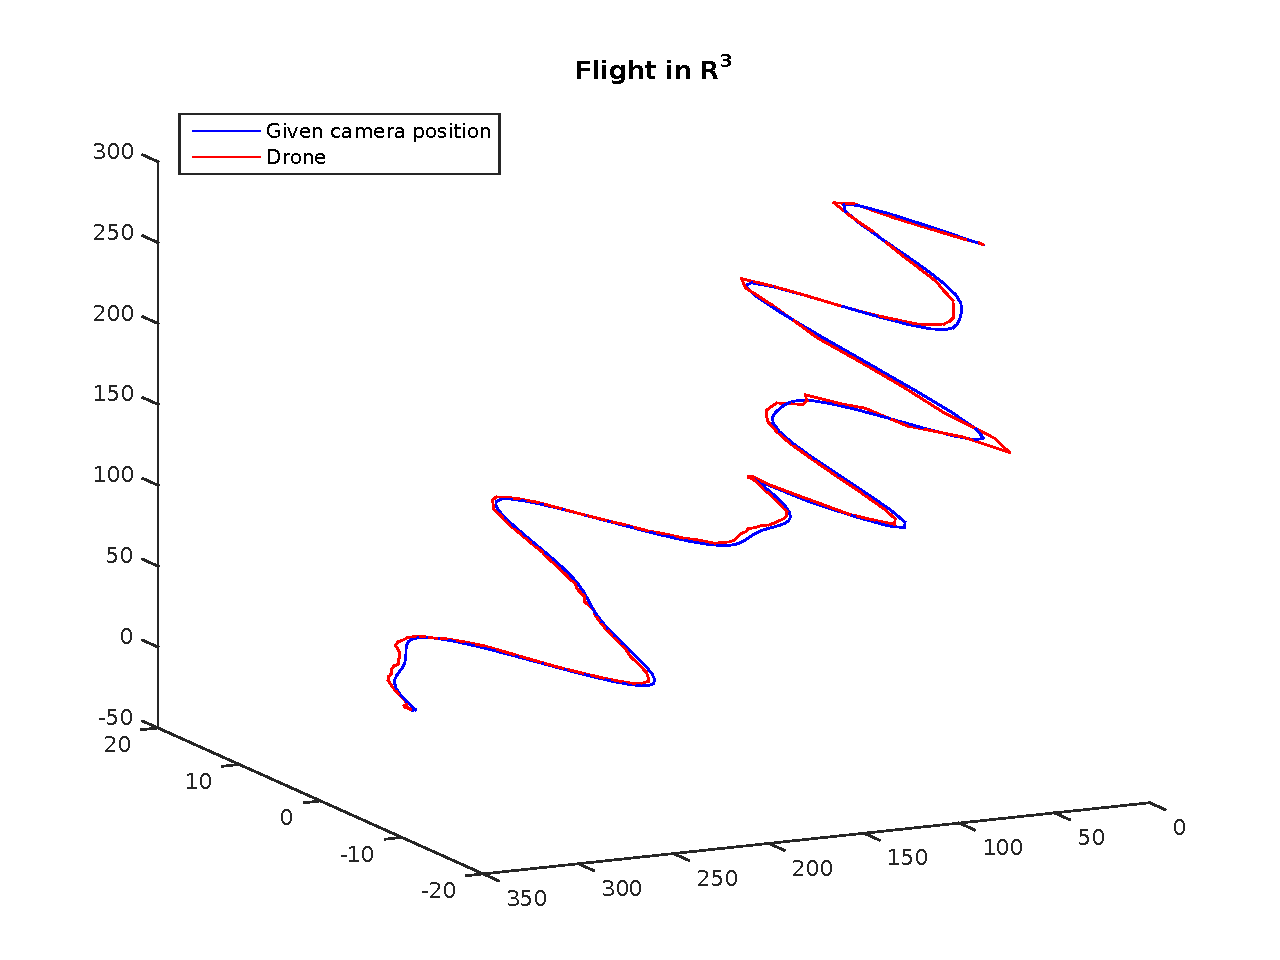
\includegraphics[width=0.9\columnwidth]{images/r3Plot.pdf}
	\end{figure}
\end{frame}

\begin{frame}
	\frametitle{Following a Skier}
	\begin{figure}
		\centering
		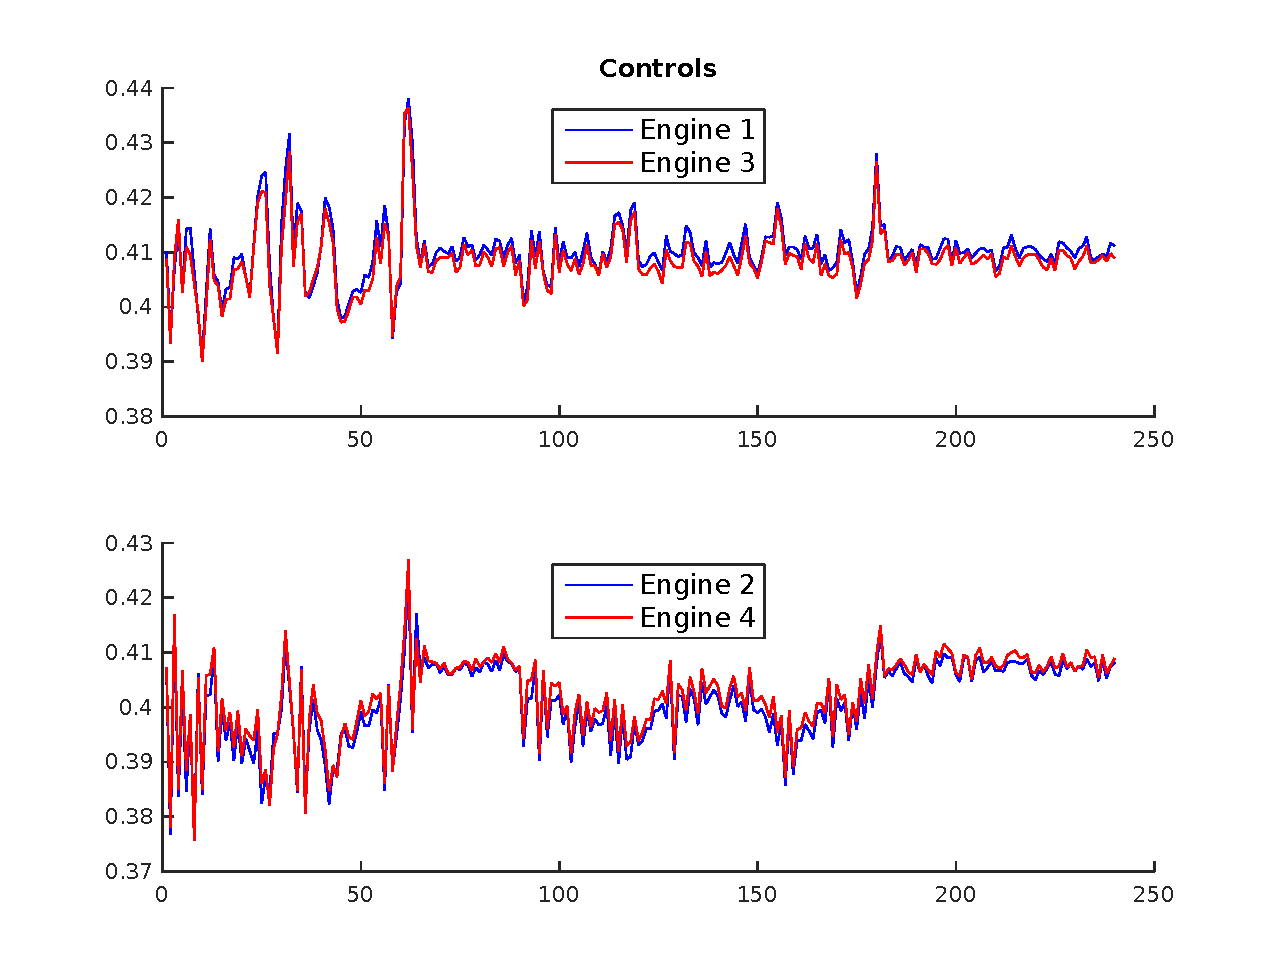
\includegraphics[width=0.9\columnwidth]{images/neu/controls.pdf}%
	\end{figure}
\end{frame}

\begin{frame}
	\frametitle{Approximations}
	\begin{figure}
		\centering
		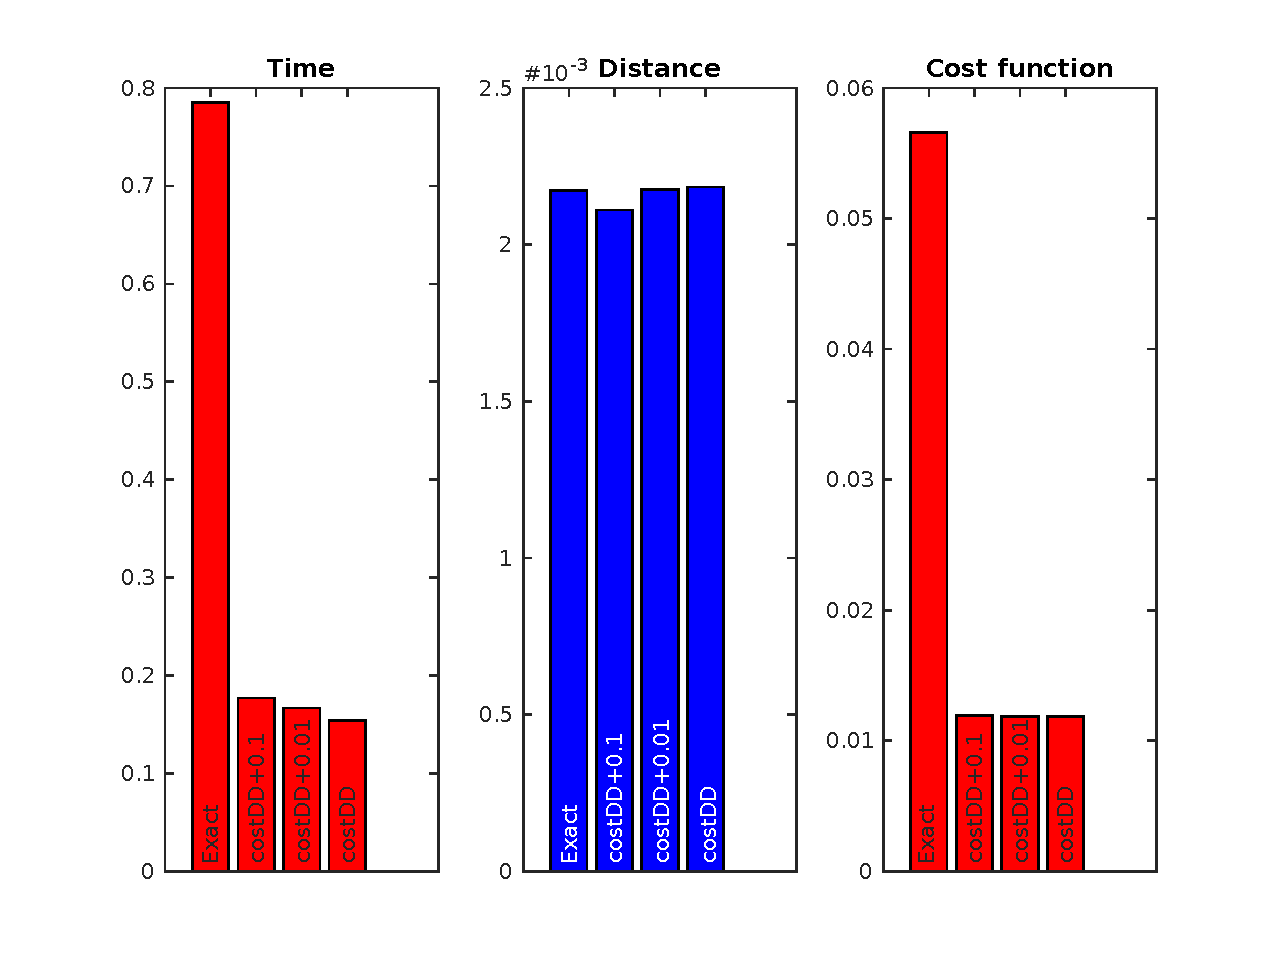
\includegraphics[width=0.9\columnwidth]{images/approxPlot.pdf}%
	\end{figure}
\end{frame}